\documentclass[12pt,letterpaper]{article}
\usepackage[utf8]{inputenc}
\usepackage[spanish]{babel}
\usepackage{amsmath}
\usepackage{amsfonts}
\usepackage{amssymb}
\usepackage{graphicx}
\usepackage{ragged2e}
\usepackage{cite}
\usepackage{float}
\usepackage{wasysym}
\usepackage{subfig}
\graphicspath{ {imagenes/} }
\usepackage{amsmath, amsfonts, amssymb}
\usepackage[left=2.5cm,right=2.5cm,top=2cm,bottom=2cm]{geometry}
\author{Javier Said Naranjo Miranda\\ Grupo: 2CM4}
\title{Teor\'ia Computacional\\ Regular Expressions}
\date{17 de octubre de 2016}
\begin{document}
\maketitle
\justify
La expresi\'on regular a trabajar sera la siguiente $L(A)= (0+1)^*01$, a continuaci\'on se mostrara el diagrama del aut\'omata no deterministico de la expresi\'on regular.

\begin{figure}[H]
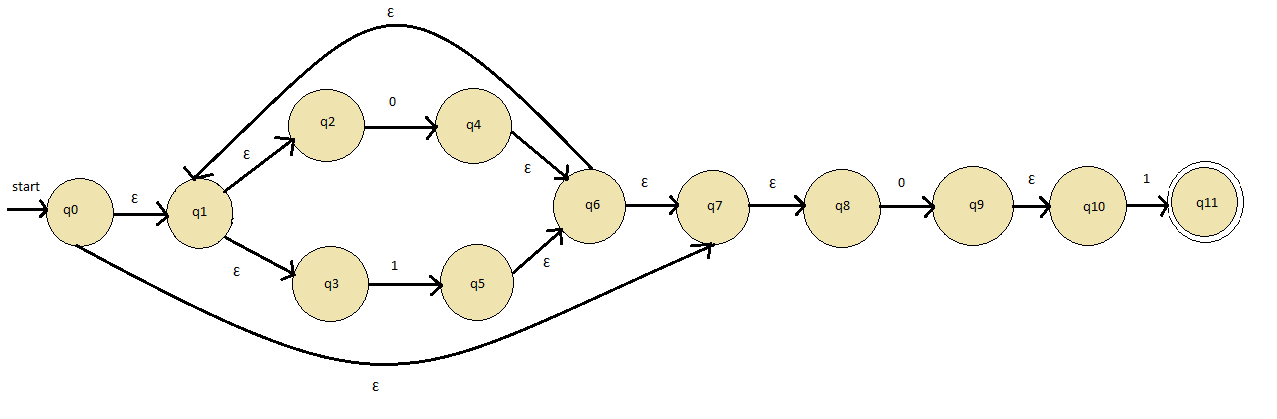
\includegraphics[width=\textwidth, height=10cm]{RE1.png}
\label{fig: RE}
\caption{Diagrama del aut\'omata no determinista}
\end{figure}

\justify
A continuaci\'on se mostraran las clausuras$_\epsilon$ para hacer la equivalencia entre aut\'omata no determinista y aut\'omata  determinista.\\
$Clausura_\epsilon(q0)=\{q0,q1,q2,q3,q7,q8\}$\\
$Clausura_\epsilon(q4)=\{q4,q6,q7,q8,q1,q2,q3\}$\\
$Clausura_\epsilon(q5)=\{q5,q6,q7,q8,q1,q2,q3\}$\\
$Clausura_\epsilon(q9)=\{q9,q10\}$\\

Ahora se mostrara la tabla para la construcci\'on de dicha equivalencia entre aut\'omatas.\\

\begin{center}
\begin{tabular}{| c || c | c |} \hline
 & 0 & 1  \\
\hline\hline
$\phi$ & $\phi$ & $\phi$ \\
\hline
$\rightarrow$ $\lbrace q0,q1,q2,q3,q7,q8 \rbrace$ & $\lbrace q4,q6,q7,q8,q1,q2,q3,q9,q10 \rbrace$ & $\lbrace q5,q6,q7,q8,q1,q2,q3 \rbrace$ \\
\hline
$\lbrace q4,q6,q7,q8,q1,q2,q3,q9,q10 \rbrace$ & $\lbrace q4,q6,q7,q8,q1,q2,q3,q9,q10 \rbrace$ & $\lbrace q5,q6,q7,q8,q1,q2,q3,q11 \rbrace$ \\
\hline
$\lbrace q5,q6,q7,q8,q1,q2,q3 \rbrace$ & $\lbrace q4,q6,q7,q8,q1,q2,q3,q9,q10 \rbrace$ & $\lbrace q5,q6,q7,q8,q1,q2,q3 \rbrace$\\
\hline
$* \lbrace q5,q6,q7,q8,q1,q2,q3,q11 \rbrace$ & $\lbrace q4,q6,q7,q8,q1,q2,q3,q9,q10 \rbrace$ & $\lbrace q5,q6,q7,q8,q1,q2,q3 \rbrace$ \\
\hline
     
\end{tabular}
\end{center}
\justify

Para hacer la equivalencia entre el aut\'omata finito determinista y el no determinista, es necesario hacer la construcci\'on de los subconjuntos del conjunto de estados.\\
A continuaci\'on se muestra el etiquetado de cada uno de los subconjuntos.\\
\begin{center}
\begin{tabular}{| c | c |} \hline
Subconjunto & Etiqueta \\
\hline\hline
$\phi$ & \textit{A} \\
\hline
$\lbrace q0,q1,q2,q3,q7,q8 \rbrace$ & \textit{B}  \\
\hline
$\lbrace q4,q6,q7,q8,q1,q2,q3,q9,q10 \rbrace$ & \textit{C} \\
\hline
$\lbrace q5,q6,q7,q8,q1,q2,q3 \rbrace$ & \textit{D} \\
\hline
$\lbrace q5,q6,q7,q8,q1,q2,q3,q11 \rbrace$ & \textit{E} \\
\hline
     
\end{tabular}
\end{center}

A continuaci\'on se muestra la tabla de transiciones del aut\'omata no determinista con el reetiquetado correspondiente. De esta manera obtenemos la equivalencia entre el AFN y el AFD.\\

\begin{center}
\begin{tabular}{| c || c | c | } \hline
 & 0 & 1 \\
\hline\hline
\textit{A} & \textit{A} & \textit{A} \\
\hline
$\rightarrow$ \textit{B} & \textit{C} & \textit{D} \\
\hline
\textit{C} & \textit{C} & \textit{E} \\
\hline
\textit{D} & \textit{C} & \textit{D} \\
\hline
*\textit{E} & \textit{C} & \textit{D} \\
\hline
\end{tabular}
\end{center}
\justify
\newpage
Se muestra una imagen del diagrama del aut\'omata determinista para la expresi\'on regular.\\

\begin{figure}[H]
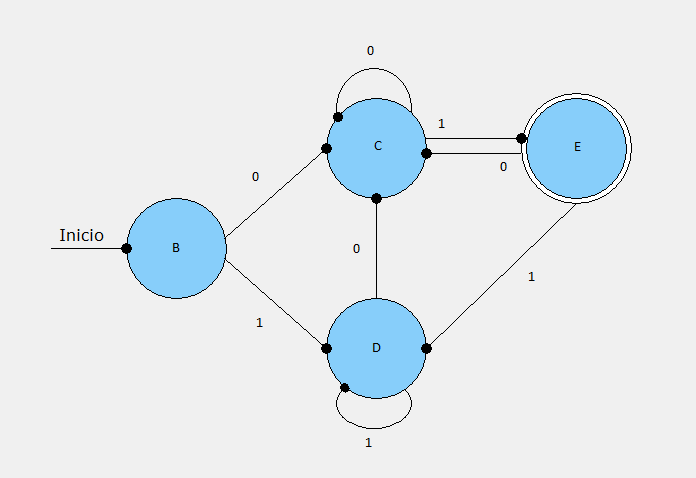
\includegraphics[width=\textwidth, height=10cm]{RE2.png}
\label{fig: busqueda}
\caption{Diagrama del aut\'omata determinista}
\end{figure}



\end{document}